%%THIS IS A SHARED GDOC. DO NOT EDIT ANY LOCAL TEX FILE VERSIONS%%

\documentclass[conference]{IEEEtran}
\IEEEoverridecommandlockouts  
% The preceding line is only needed to identify funding in the first footnote. If that is unneeded, please comment it out.
%\usepackage{cite}
\usepackage{amsmath,amssymb,amsfonts}
\usepackage{algorithmic}
\usepackage{graphicx}
\usepackage{textcomp}
\usepackage{array}
\usepackage{tabu}
\usepackage{subfig}
\def\BibTeX{{\rm B\kern-.05em{\sc i\kern-.025em b}\kern-.08em
        T\kern-.1667em\lower.7ex\hbox{E}\kern-.125emX}}
\makeatletter


\begin{document}
    
    \title{OpenPodCar: an open source vehicle for self-driving car research \\
        \thanks{This project has received funding from EU H2020 interACT: Designing cooperative interaction of automated vehicles with other road users in mixed traffic environments under grant agreement No 723395. Thanks to Yao Chen for making figures X and Y, and Gabriel Walton for scoping simulation tools.}
    }
    
    
    \author{
        \IEEEauthorblockN{Chris Waltham\IEEEauthorrefmark{2}, Fanta Camara\IEEEauthorrefmark{1}\IEEEauthorrefmark{2},David Churchill\IEEEauthorrefmark{2}, Charles W. Fox\IEEEauthorrefmark{1}\IEEEauthorrefmark{2}}
        \IEEEauthorblockA{\IEEEauthorrefmark{1}Institute for Transport Studies, University of Leeds, UK}
        \IEEEauthorblockA{\IEEEauthorrefmark{2} School of Computer Science, University of Lincoln, UK}
   %     \IEEEauthorblockA{\IEEEauthorrefmark{3} Ibex Automation Ltd., UK}
    }
    
    
    
    \maketitle
    
    \begin{abstract}
        
Open source software for autonomous vehicle (“self driving car”) control is now available but there is a need for a corresponding open-source hardware platform to enable researchers to build standard setups and share research in this field.   Here we are constructing such a platform.   The Lincoln Podcar is a physical vehicle based on a low cost off the shelf, hard canopy, mobility scooter.  It is large enough to transport one person at speeds up to 15kmh, for example for use as a last-mile autonomous taxi service from the train station to the office; or to transport up to three Deliveroo-sized freight containers similarly around a city center. But it is also small enough to make serious injury to pedestrians unlikely in the event of a collision.  Together with its low costs it thus forms an ideal balance between real world utility, safety, cost and resarch convenience.  The open source platform consists of (a) CAD designs, sample bill of materials, and build instructions to modify the off the shelf donor vehicle for electronic control; (b) Arduino, ROS and Gazebo control and simulation software files which provide standard ROS interfaces and simulation of the vehicle; and (c) higher-level ROS implementations of standard medium-level robot control, including the movebase interface which enacts command to get the vehicle from one pose to another.  The vehicle uses Ackermann steering and Reeds-Sheppe curves.   Its total build cost in 2020 is around 7000USD in total, including sensors and computing equipment.

 
    \end{abstract}    
    
    \begin{IEEEkeywords}
        Autonomous Vehicles,  Pedestrian - Vehicle Interaction
        [3 maximum]
    \end{IEEEkeywords}
    

    \begin{figure}[h]
      \includegraphics[width=\columnwidth]{hardware/testDrive.png}
      \caption{OpenPodcar test drive.}
      \label{fig:testDrive}
    \end{figure}

    \section{Requirements}
 
Specific requirements for such a platform are that it needs to be as low cost as possible, and easy to build.  This is to enable the community to reproduce and use it.   Consumer levels of safety and reliability are not required, preferring to minimise cost, through research standards of safety and reliability are required.
    
\section{Donor vehicle}    
A PIHSIANG TE-889XLSN hard-canopy scooter (branded in UK as Shoprider Traverso) is used as the pod car platform. It is an electric car powered by two 12V batteries connected in series to provide 24V operating voltage and containing 75Ah. Its steering is controlled by human operated loop handle bar.  Speeding and braking system are both powered by an electric motor and an electric brake via the trans-axle assembly, controlled by AC2 digital controller receiving different voltage signals to drive forward or brake. The manual speeding and braking systems were controlled by three buttons connected in series on the handle bar: A toggle switch in parallel with a resistor (10kΩ) to choose speed mode high or low; A speed dial knob via a variable resistor (20kΩ) to choose a maximum speed value; A throttle lever connected with a potentiometer (5kΩ), 2.5kΩ to 2.6kΩ for each side to speed or brake. 

\section{Mechanical modification}

\subsection{Steering}
To automate steering, a GLA750-P 12V DC linear actuator with position feedback is mounted under the chassis to car's front axle via bearings.  This actuator has a 8mm/s full load (750N) speed and 250mm stroke length (installation length is 390mm). 
To access the underside of the vehicle, use two
 axle stands TODO photo.

There is an existing hole in the right front wheel axle.  Mount the linear actuator via rear hole to the left side of front chassis and connect it through the front hole of the actuator with the hole in the car's right front wheel axle via bearings as shown in Fig. \ref{fig:steering}. 

    \begin{figure}[h]
      \includegraphics[width=\columnwidth]{hardware/onAxles.jpg}
      \caption{Tilting the vehicle using two axle stands, to enable access to the underside. (Note also lidar mounted to roof.)}
      \label{fig:axelStands}
    \end{figure}

    \begin{figure}[h]
      \includegraphics[width=\columnwidth]{hardware/steeringActuatorMounted.jpg}
      \caption{Underside with linear actuator added for steering.}
      \label{fig:actuatorMounted}
    \end{figure}

\subsection{Sensors}
\subsubsection{Lidar}
Velodyne16 lidar sensor.  Mounted on the vehicle roof using a small optical tripod (TODO give model). Note that optical devices have unusual physical mounting standards which use Imperial rather than metrics units.  This system is used by optics research based on optical table sizing.   The lidar screws onto the tripod. The tripod is cabled-tied to the vehicle roof via  drilled holes at locations in fig. TODO.  It is mounted at a 10 degree tilt downwards (to allow pedestrians to be most clearly seen in the 16 scan lines).

\subsubsection{Odometry}
TODO -- we need some hall effect or other shaft encoders to measure odometry.

\section{Electronic modification}


    \begin{figure}[h]
      \includegraphics[width=\columnwidth]{hardware/pic_boards.jpg}
      \caption{Below-seat area inside cabin, with newly added boards..}
      \label{fig:actuatorMounted}
    \end{figure}


    \begin{figure}[h]
      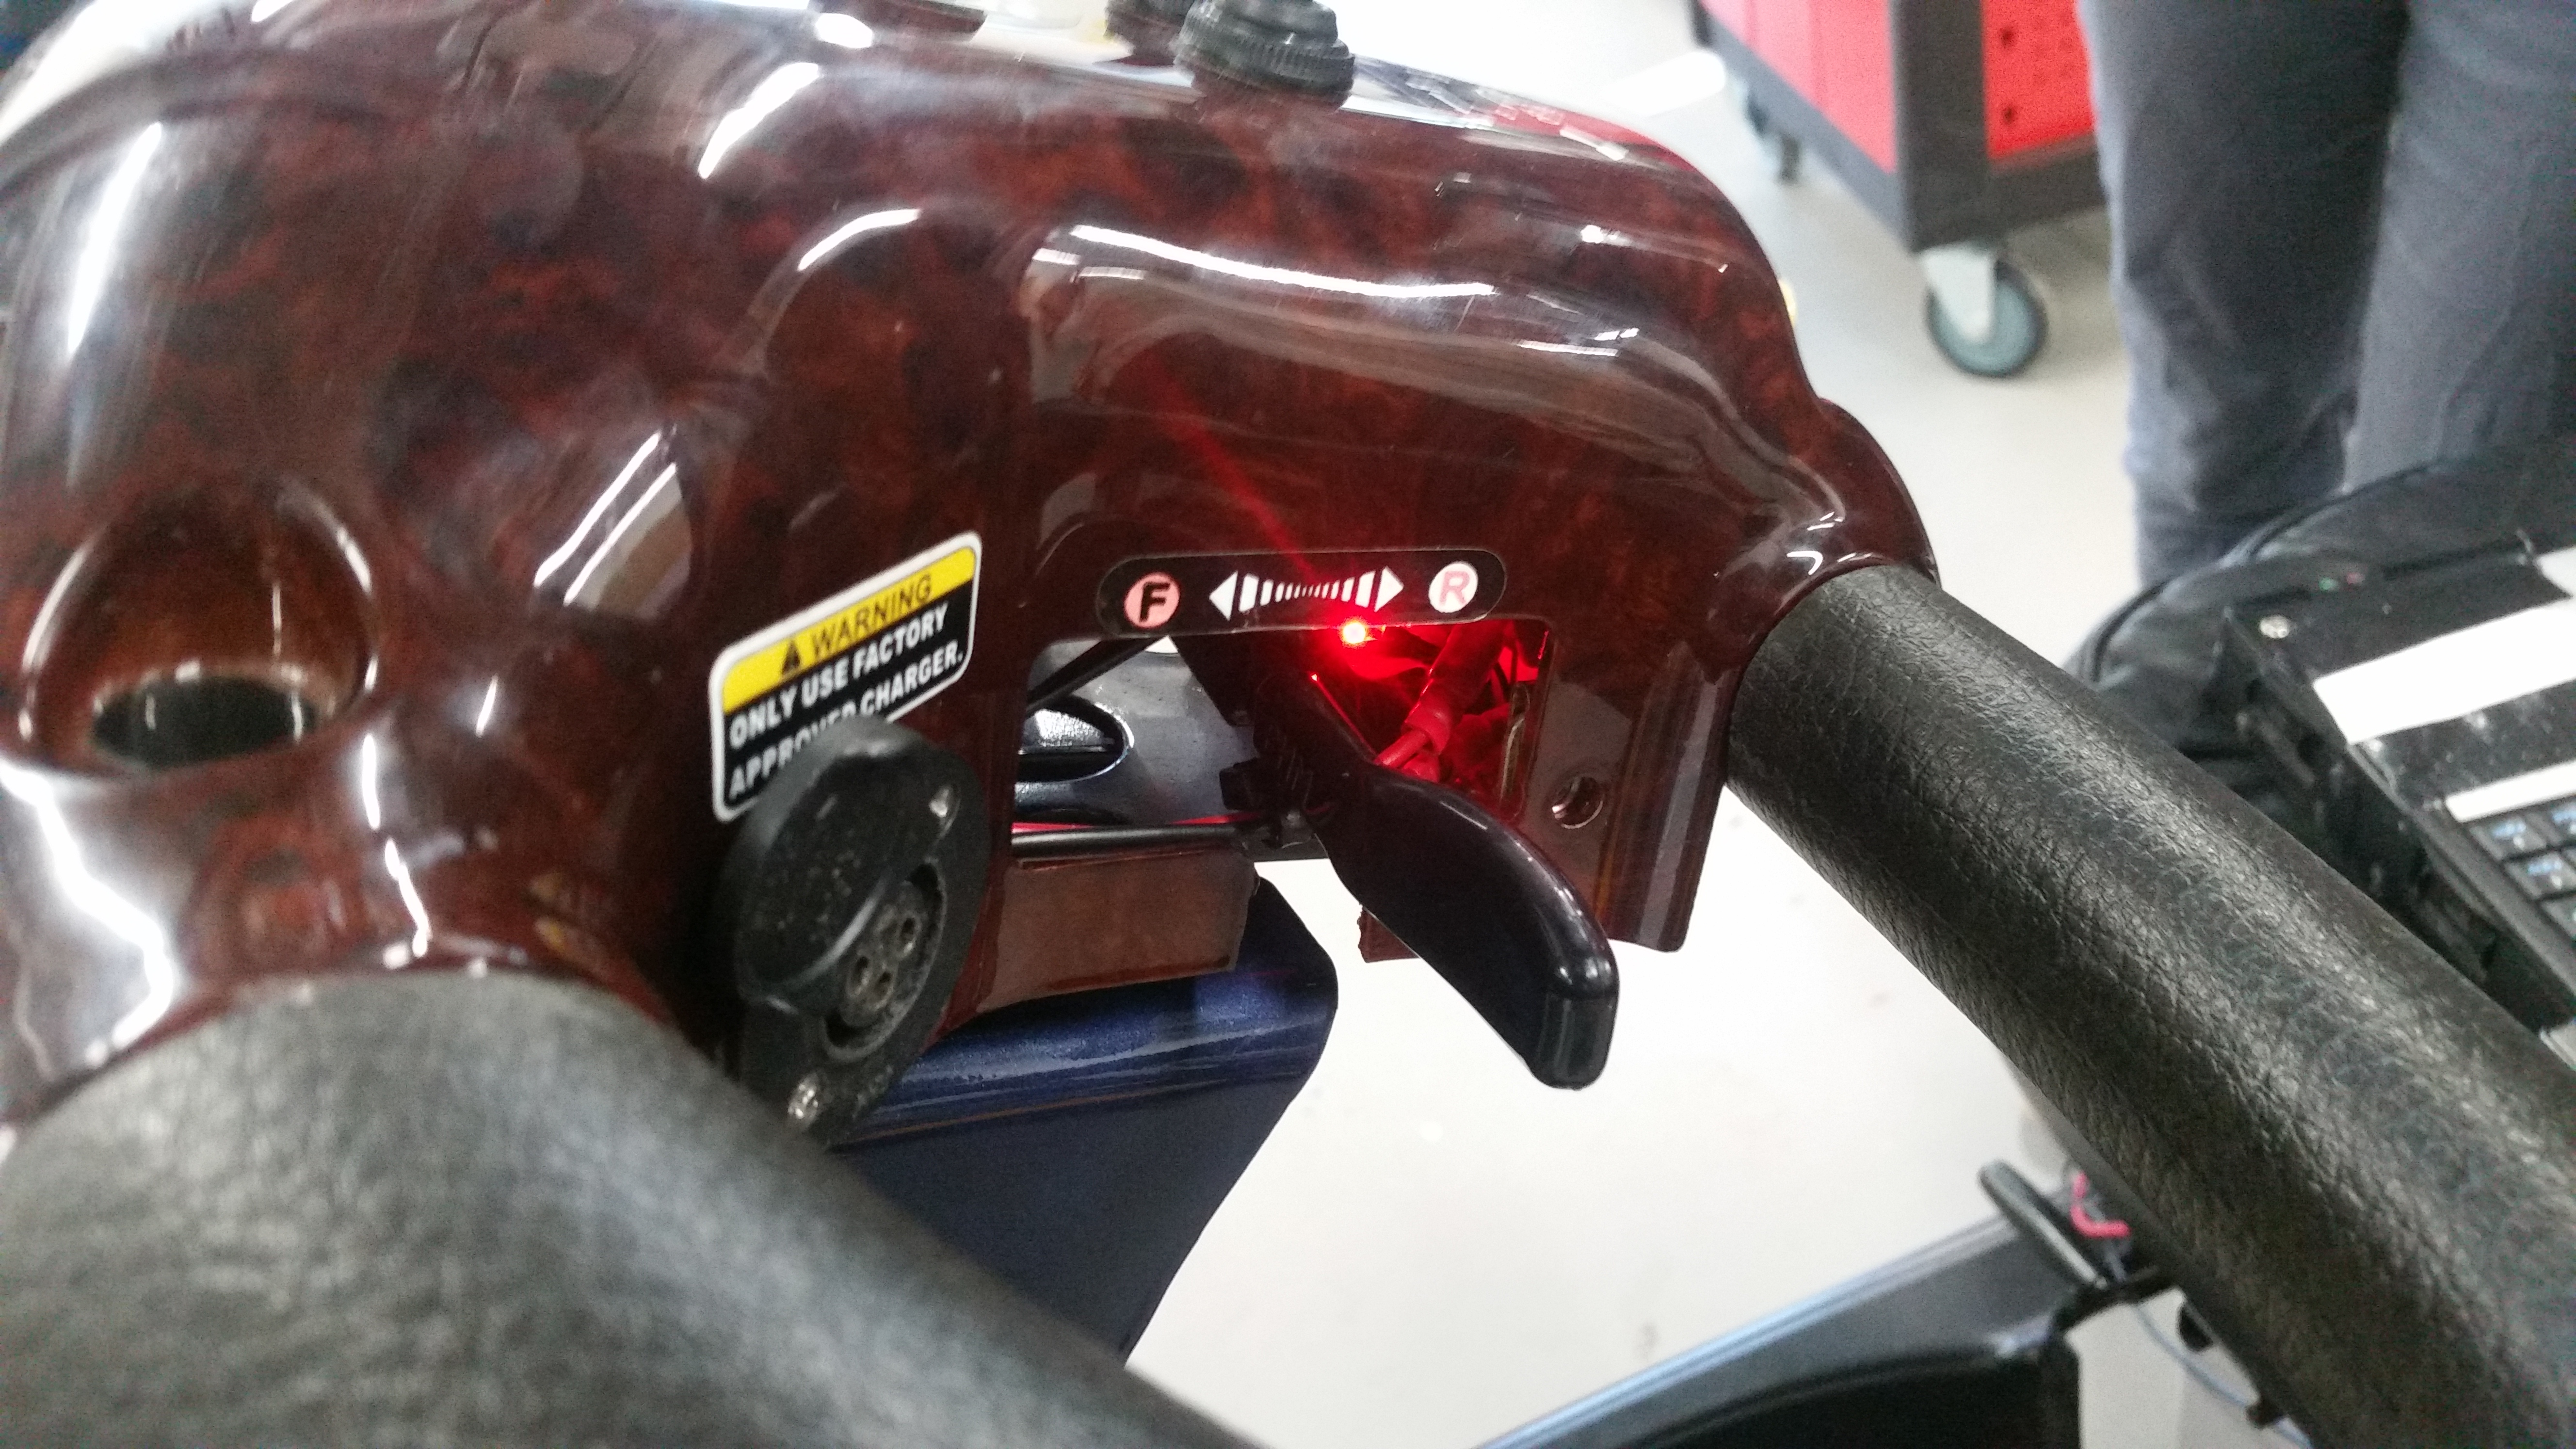
\includegraphics[width=\columnwidth]{hardware/pic_relay.jpg}
      \caption{Steering console showing newly added relay (with lit LED) to dead man’s handle, replacing the ignition switch (only) in the circuit.}
      \label{fig:actuatorMounted}
    \end{figure}


    \begin{figure}[h]
      \includegraphics[width=\columnwidth]{hardware/circuitDiagram.png}
      \caption{Circuit diagram for electronic modifications.}
      \label{fig:circuitDiagram}
    \end{figure}
    
    \begin{figure}[h]
      \includegraphics[width=\columnwidth]{hardware/drilling.png}
      \caption{Drilling.}
      \label{fig:drilling}
    \end{figure}


\subsection{Steering}

The front wheels are steered by a Pololu (TODO give model number)  PID controller, which takes serial port desired positions as input. It also takes feedback position information as an analog voltage from the linear actuator as an input. It outputs analog high-power voltages to the linear actuator.

TODO give PID settings.Windows app is needed to set them once only.


The relationship between the required central turning angle $\theta$ of the pair of front wheels and extending length $l$ of linear actuator is,    
    \begin{gather}
    \theta = \alpha - \arctan(\frac{W}{2H}) \\
    % update W and H in figure. W is the width between two front wheels and H is the distance between front wheel and rear wheel.
    \beta = \alpha -\frac{\pi}{2}\\
    x = r_1 * \cos(\beta) \\
    y = r_1 * \sin(\beta) \\
    l = \sqrt{(x_0-x)^2 + (y_0-y)^2} - L + l_0    
    \end{gather}    
    Where $r_1$, $x_0$, $y_0$, $W$, $H$ and $L$ are the geometric coefficients shown in Fig.1. Among them, the value of $y_0$ is negative. $l_0$ is the initial value of the linear actuator position feedback.

    \begin{figure}[h]
      \includegraphics[width=\columnwidth]{hardware/steering1.png}
      \caption{The bottom view of front wheels steering relationship including geometric coefficients}
      \label{fig:steering}
    \end{figure}
    
    % related to:
    %'889XLSBN CAN Traveso Spare Parts List' page 29, 30, 32, 33, 34, 37, 38, 40 and 41;
    %'Shoprider Scooter Service Manual Live Document' page 7, 8, 14 and 16.
   

Test commands can be passed to the Pololy using the commands in /tools/cmdSteer **DO NOT GIVE COMMANDS OUTSIDE RANGE 1000-25000 AS THEY HAVE DAMAGED THE VEHICLE**.  TODO -- WRITE SAFETY WRAPPER FOR THIS.

A non-ROS test of the C API for the Pololu is is /tools/pololuTestCSerial.    


    \begin{center}
        \begin{tabular}{ c c }
            \hline
            FA:cmd     &  Effect \\
        2500    &    max right  \\
        1900    &    center  \\ 
        1000    &    max left  \\
            \hline\\
        \end{tabular}
    \end{center}    

 **DO NOT SEND COMMANDS OUT OF THS RANGE AS THEY HAVE MECHANCIALLY DESTROYED THE SYSTEM**


    
\subsection{Speed}

\subsubsection{Dead man’s handle - IMPORTANT SAFTEY INFORMATION}

Autonomous vehicles can present a significant hazard to people and the environment in which they operated. Damage to surroundings and possible injury to operators and bystanders could result from inappropriate use or malfunction. It is essential that a suitable emergency stop system is implemented in all autonomous vehicles.

Implementing and testing this safety system should be undertaken with the drive wheels of the vehicle raised off of the ground, allowing for checks to be made of the DMH without the risk of the vehicle speeding off out of control.

Given the development platform nature of the OpenPodCar, a safety mechanism which stops the vehicle under fault conditions is a very important part of the design. During the build several methods of implementing this safety system where checked, the one described below is the current solution.

The speed controller on this particular mobility scooter has a dead zone at around 2.5V on its speed input signal which corresponds to drive wheels stopped. Above the dead zone and up to 5V being forward control values and 0V to below the dead zone being reverse control voltages.

These values were checked using a multi meter prior to implementing the Arduino controller and DAC.
This means that if the DAC output from the Arduino where to fail and 0V for example is applied to the mobility scooters speed controller input, the vehicle would respond by spinning the drive wheels backwards at full throttle. This being a dangerous eventuality, it is very important in terms of safety to ensure this situation can not arise.

A two stage approach is used to reduce this risk. Please refer to the schematic diagram DMH section in conjunction with this description.

\paragraph{Stage 1 – The Relay.} A relay is used which interrupts the mobility scooter’s key ignition circuit. If the relay is not energised by the presence of a 5V supply to the Arduino, the vehicles movement is disabled. This effectively ensures that if the Arduino is non-functional, for example its power supply has failed or it has been unplugged from the USB port of the control PC and there is a danger that the DAC is not producing the control systems required voltage, the scooter is automatically disabled by effectively switching it off.

\paragraph{Stage 2 – The DMH Switch.} A sturdy push button is used which also interrupts the vehicles key ignition circuit. If the PodCar operator detects any abnormality in operation during operation, he/she simply releases pressure from the DMH switch and the vehicles movement is disabled. The DMH switch is wired in series with the relay in the key ignition circuit ensuring that if both the relay contacts and the DMH switch are closed, this is the only condition where the PodCar movement is active.
The addition of the Relay and the DMH Switch are essential for safe operation, especially where new unproven autonomous control systems are in development.





Deadman’s handle to ignition. Replace key with relay (TODO model) and dead-mans-handle button switch (TODO model) on a 10m, 2-core cable.    TODO: are any other console functions changed? 

TODO edited version of wiring from shoprider manual. And photo of the real wires.

\subsubsection{Speed control}

TODO how to set the console switches to correct fixed settings.

Arduino UNO is used to send electric signals to vehicle's motor controller instead of using speed buttons.  TODO DAC model and wiring.  TODO arduino wiring.

Arduino code is supplied in the distribution (/Arduino/ThrottleControlSerial.ino). When uploaded to the Arduino (using the standard Arduino IDE running on the laptop), it provides a simple serial port API running at 112000baud (TODO other erial options.)  It receives commands of the form “FA:210” as speed commands.   The test scripts /tools/zeroSpeed.py and /tools/testSpeed.py can be used to send example commands for debugging.

    \begin{center}
        \begin{tabular}{ c c c }
            \hline
            FA:cmd &      Voltage            &  Effect \\
        0    &    0        & stupid fast reverse  \\
        80    &    0        & v fast reverse (ros limit) \\
        132    &    1.82        & slowest reverse motion  \\
            &            & stop - dead zone - allows signition \\
        201    &    2.71        & slowest forward motion \\
        240    &    2.78        & v fast forward (ros limit) \\
        255    &    ?        & stupid fast forward \\
            \hline\\
        \end{tabular}
    \end{center}    

To start the ignition, car safety system required the control vltage to be in the dead range.
Problem is this doesnt correposnd to fixed speedbytes due to the USB power issues.
But if we pick a number solidly in the center of the deadzone, such as 164, then it will be OK for most USB supplies.

when battery is flat, the voltages are lower? eg send 164 and get 1.9V instead of 2.26V ?
this may result in vehicle not starting - maybe by design or accident. get beep as is outside start zone.
thoery: the ardunio is getting lower power eg max 4.9V instead of 5V, which gets divided by the DAC value.  To deal with these instabilities, we added a potential divider at the battery to check the voltage and control the podcar accordingly.

      \begin{figure*}[h]
      \includegraphics[width=\textwidth]{potential_divider.png}
      \caption{Potential divider linked to the battery}
      \label{fig:potential_divider}
    \end{figure*}




    \begin{itemize}
        \item insert Figure 2 about the wiring diagram of speed buttons and micro-controller.
        \item talk about safety (dead-man button).And speed code part with details.\\
    \end{itemize}    

\section{Lidar setup}
velodyne works with the velodyne ROS package. But it needs to be set up so we can talk to the Velodyne over ethernet.  The laptop must be on wired network, not wifi.   The IPs must be configured as in the velodyne docs TODO details/refs.  The lidar IP is 192.168.1.201.


\section{ROS inferface}
For ROS Kinetic and Ubuntu 16.04 (xenial), standard in robotics research.


    \begin{figure*}[h]
      \includegraphics[width=\textwidth]{software/rosnodes.png}
      \caption{ROS nodes and messages for low level control.}
      \label{fig:meshSim}
    \end{figure*}


\section{Simulation}


    \begin{figure}[h]
      \includegraphics[width=\columnwidth]{software/podcar_phys_sim.png}
      \caption{Physical simulation of vehicle.}
      \label{fig:physSim}
    \end{figure}

    \begin{figure}[h]
      \includegraphics[width=\columnwidth]{software/podcar_mesh.png}
      \caption{Visual mesh simulation of vehicle.}
      \label{fig:meshSim}
    \end{figure}




A robotics simulation of the vehicle is provided for use in Gazebo 8.6.0 underROS Kinetic and Ubuntu 16.04 (Xenial).

The physics simulation is based on a simplified vehicle geometry with two large cuboids containing the vehicles’ mass. \ref{FIG} Parallel steering linkage is simulated via ODE joints forming a tracking rod. Rear drive motor and the steering linear actuator are simulated via ODE PID controllers.  Wheel geometry was measured from the physical vehicle.   Wheel forwards and lateral Coulomb friction coefficients were tuned by trial and error to produce realistic motion and steering.  The model is represented in SDF format, which is easy portable for use in other simulation and CAD systems.

There are some key differences when it comes to actuating the tracking rod between simulation and real life. On the physical robot, a linear actuator is mounted on the underside of the vehicle and attached to the front axle, which can extend/retract to angle the wheels. However, in simulation, the pivot joints that join the front wheels and the tracking rod can have a force applied directly to them without the need for a complicated actuator. This reduces the complexity of the model without affecting its behaviour, and is still appropriately accurate to real life.

There are also some similarities, for example both steering solutions implement a PID
(Proportional, Integral, Derivative) controller, that uses a proportional gain, integral function
and differential function to determine exactly how much force to apply at any given time in
order to keep the wheels at the desired angle. The parameters for the existing robot’s PID
controller have not been published, however trial and error found a proportional gain of 2,
differential weight of 1 and integral weight of 0 were adequate.

The simulation implements the same ROS interface as the physical vehicle system to enable plug and plug interoperability between them.  In the simulation, vehicle control messages are recevied, and vehicle sensor messages are sent by, a Gazebo plugin (podcarGazeboROSPlugin.cpp) which calls Gazebo’s simulation functions.  

Desired vehicle control commands, as for the physical vehicle, consist of (speed, angle) pairs, to command the speed of the rear wheels in m/s (speedcmd_meterssec message) and the steering angle (wheelAngleCmd message) of the front wheels in radians.  The plugin and Gazebo implement these commands using simulated rotary and linear PID controllers and actuators, to rotate the rear wheels and linearly actuate the tracking rod respectively.

The plugin then publishes sensor messages corresponding to those from the physical vehicle. These include:  /odometry/groundTruth, a (noiseless) standard odometry format estimate for the vehicle’s pose; and /camera/image_raw and /camera_depth, the depth camera data.


A detailed graphical mesh model of the vehicle is provided for display, rather than physical simulation, purposes \ref{FIG}.  This may be important for experiments such as virtual reality interactions between the simulated vehicle and human subjects, e.g. \cite{TODOFANTAVR} as their psychological responses may depend on the apparent size and share of the vehicle.

Fig. \ref{fig:sim_nodes} shows the complete ROS node configuration used during simulation, under manual joystick control.

\begin{figure}[h]
      \includegraphics[width=\columnwidth]{figs_sim/sim_nodes.png}
      \caption{ROS nodes used in simulation under manual joystick control.}
      \label{fig:sim_nodes}
\end{figure}


To install and run the simulation:
\begin{verbatim}
cd <install location>/catkin_ws
catkin_make
source devel/setup.bash
cd src/podcar/models/plugins
cmake .
make
export GAZEBO_PLUGIN_PATH=$GAZEBO_PLUGIN_PATH`pwd`:
cd ..
export GAZEBO_MODEL_PATH=$GAZEBO_MODEL_PATH`pwd`:
cd ../../../
rosdep install --from-paths src --ignore-src -r -y
roslaunch podcar podcarsim.launch
\end{verbatim}


\section{Path planning and control integration (movebase)}

Front-wheel-steering means that the front two wheels are used to steer the vehicle, with the rear wheels trailing and-or powering the vehicle.  Ackermann steering is a special case of front-wheel-steering, in which the front wheels are connected to a tracking rod via two shorter steering arms arranged so that the two steering arms form a triangle with the center point of the vehicle’s rear axle when the wheels are facing forwards.  This results (TODO cite proof) in the front wheels forming the correct angles (which are different from each other) needed for the vehicle to drive in circular segments, with the circle radius determined by the steering angle.   Vehicles whose possible driving motions are of this form are called Dubins Cars if they can drive only forwards, or Reeds-Shepp cars if they can drive forwards and reverse. ubins and Reeds-Shepp cars have possible driving trajectories from pose A to pose B which consist of at most one circle arc segment and two straight lines to and from it. The donor podcar is a Reeds-Shepp car with Ackermann steering.

    \begin{figure}[h]
      \includegraphics[width=\columnwidth]{hardware/ackermann1.png}
      \caption{Ackermann steering (Source: Wikipedia; Ackermann Steering; Creative Commons.}
      \label{fig:ackermann1}
    \end{figure}

    \begin{figure}[h]
      \includegraphics[width=\columnwidth]{hardware/ackermann2.png}
      \caption{Ackermann steering (Source: Wikipedia; Ackermann Steering; Creative Commons.}
      \label{fig:ackermann1}
    \end{figure}

Fig. \ref{fig:sim_nodes} shows the complete ROS node configuration used during movebase, with the simulation backend.  When using the physical vehicle, simulation nodes are replaced by the physical vehicle nodes as described above.

\begin{figure}[h]
      \includegraphics[width=\columnwidth]{figs_sim/sim_movebase_nodes.png}
      \caption{ROS nodes used in simulation under move_base control.}
      \label{fig:sim_movebase_nodes}
\end{figure}

\section{Localisation and mapping system}

gmapping -- current

TODO:

OrbSLAM -- based on Octomap, adding mono visual features.  
Octomap can also be used with any other point cloud data eg lidar.

NDT SLAM -- used at LCAS - ILIAD.

\section{User Guide}    

\subsection{Power up}
Check that the vehicle’s original lever for auto-manual is set to auto (DOWN). It is on the main motor, under the vehicle at the rear left, colored red. Requires some force to move it.

Power on the vehicle using the original on-off switch located under the seat on the left. It is marked ON-OFF.

Power on the modified electronics using the new toggle switch.   (This lights LEDs on the DCDCs and Pololu, and the lidar makes a whirring sound).

Check that the batteries are charged (use a multimeter across one of the DCDC converters, need to see 24V or over. DO NOT USE THE VEHICLE IF IT IS UNDERCHARGED, THIS IS DANGEROUS.

Power on the laptop using the slider switch on its front right.

Login as user podcar, password TODO.

Type:  roscd podcar

Unplug the laptop’s USB connection and plug it in again.  (HACK)

Run the test script podcar/tools/pololuCSerialTest/a.out  (HACK)

Type: roslaunch podcar podcar.launch

Use the joystick to control steering and speed.

\subsection{Usage}


\section{Troubleshooting Guide}

\subsection{Vehicle}
\subsubsection{vehicle beeps continuous when press DMH and rear wheels do not move}
This is due to a safety mode preventing ignition.

Check: is the manual-auto switch under the rear motor on auto?

Check: are the batteries well charged (must be 24V or over.)

Check: is the control voltage is the dead zone, it should be.

\subsubsection{Rear wheels do not move, control voltages are correct}
Control voltages means the display on the voltmeter LED. Should be above 1.2 or below 1.8 for forward and backwards.

Check: main vehicle battery level, by connecting the vehicle charger and inspecting the battery charge level. Problem occurs if battery is nearly flat.

Check: charger must be disconnected for rear wheels to moe (safety feature).


\subsection{Lidar}
\subsubsection{No velodyne_points message published}
Check: laptop must be on wired network, not wifi.

Check: wired network must be configured correctly, see velodyne setup docs. Maybe be interfered if wifi has been used recently.  Check connections to velodyne box including power and ethernet.
   


\subsection{Simulation}
\subsubsection{AF_NET error}
If this is thrown by the Gazebo plugin -- it may be because Gazebo is being run standalone rather than launched as a ROS node as required.




 \section{Related work}
 About 20 references or more if you can (at least one page) about similar work, SLAM, vehicle control and simulation, open source projects....  Cite this project from UC berkeley: http://www.barc-project.com/ 
 
    
    
\section{Discussion}
We hope that the platform will be useful...

    
\section{Acknowledgements}
Thanks to Jacob Lord for creating the graphical mesh model, and Yao Chen for initial research into Dubins path methods.
    
    \bibliographystyle{plain}
    \bibliography{references_podcar}
    
\end{document}








